% Created 2016-05-12 Thu 21:25
\documentclass[10pt,oneside,x11names]{article}
\usepackage[utf8]{inputenc}
\usepackage[T1]{fontenc}
\usepackage{fixltx2e}
\usepackage{graphicx}
\usepackage{grffile}
\usepackage{longtable}
\usepackage{wrapfig}
\usepackage{rotating}
\usepackage[normalem]{ulem}
\usepackage{amsmath}
\usepackage{textcomp}
\usepackage{amssymb}
\usepackage{capt-of}
\usepackage{hyperref}
\usepackage{geometry}
\usepackage{amsmath}
\usepackage{amssymb}
\usepackage{amsfonts}
\usepackage{palatino}
\usepackage{siunitx}
\usepackage{esdiff}
\usepackage{xfrac}
\usepackage{nicefrac}
\usepackage{faktor}
\usepackage[euler-digits,euler-hat-accent]{eulervm}
\author{Brian Beckman}
\date{\textit{<2016-05-03 Tue>}}
\title{Kalman Folding 5: Non-Linear Models and the EKF (WORKING DRAFT)\\\medskip
\large Extracting Models from Data, One Observation at a Time}
\hypersetup{
 pdfauthor={Brian Beckman},
 pdftitle={Kalman Folding 5: Non-Linear Models and the EKF (WORKING DRAFT)},
 pdfkeywords={},
 pdfsubject={},
 pdfcreator={Emacs 24.5.1 (Org mode 8.3.4)}, 
 pdflang={English}}
\begin{document}

\maketitle
\setcounter{tocdepth}{2}
\tableofcontents


\section{Abstract}
\label{sec:orgheadline1}

In \emph{Kalman Folding, Part 1},\footnote{B. Beckman, \emph{Kalman Folding, Part 1}, to appear.} we present basic, static Kalman filtering
as a functional fold, highlighting the unique advantages of this form for
deploying test-hardened code verbatim in harsh, mission-critical environments.
In \emph{Kalman Folding 2: Tracking},\footnote{B. Beckman, \emph{Kalman Folding 2: Tracking}, to appear.} we reproduce a tracking example from
the literature, showing that these advantages extend to time-dependent, linear
models. Here, we extend that example further to include aerodynamic drag, making the
model nonlinear. We must change the Kalman filter itself to handle such
problems. The resulting class of filters are called Extended Kalman Filters or
EKFs. Other papers in this series feature applications of EKFs to a variety of
problems including navigation and pursuit.

The particular EKF designed here includes integration of non-linear equations of
motion. We integrate these equations by folding over a lazy stream that
generates, on demand, differential updates to the solution. Folds over lazy
streams were introduced in \emph{Kalman Folding 4: Streams and Observables}\footnote{B. Beckman, \emph{Kalman Folding 3: Streams and Observable}, to appear.}
where we used them to step a static Kalman filter over observations. They also
afford a constant-memory representation for solutions of differential equations,
making them suitable for integration components in constant-memory filters.

\section{Kalman Folding in the Wolfram Language}
\label{sec:orgheadline3}

In this series of papers, we use the Wolfram language\footnote{\url{http://reference.wolfram.com/language/}} because it excels
at concise expression of mathematical code. All examples in these papers can be
directly transcribed to any modern mainstream language that supports closures.
For example, it is easy to write them in C++11 and beyond, Python, any modern
Lisp, not to mention Haskell, Scala, Erlang, and OCaml. Many can be written
without full closures; function pointers will suffice, so they are easy to write
in C. It's also not difficult to add extra arguments to simulate just enough
closure-like support in C to write the rest of the examples in that language.

In \emph{Kalman Folding 2: Tracking},\footnotemark[2]{} we found the following
formulation for the accumulator function of a fold that implements the linear
dynamic Kalman filter, that is, a filter that can track states that evolve with
time\footnote{In most applications, the independent variable is physical time,
however, it need not be. For convenience, we use the term \emph{time} to mean \emph{the independent variable of the problem} simply because it is shorter to write.} according to a linear transformation.

\begin{equation}
\label{eqn:kalman-dynamic-cume-definition}
\begin{matrix}
\textrm{kalmanDynamic}
\left(
\left\{
\mathbold{x},
\mathbold{P}
\right\},
\left\{
\mathbold{Z},
\mathbold{\Xi},
\mathbold{\Phi},
\mathbold{\Gamma},
\mathbold{u},
\mathbold{A},
\mathbold{z}
\right\}
\right) = \\
\begin{Bmatrix}
\mathbold{ x }_{ 2 }+
\mathbold{ K }\,
\left(
\mathbold{ z }-
\mathbold{ A }\,
\mathbold{ x }_{ 2 }
\right), &
\mathbold{ P }_{ 2 }-
\mathbold{ K }\,
\mathbold{ D }\,
\mathbold{ K }^\intercal
\end{Bmatrix}
\end{matrix}
\end{equation}

\noindent where

\begin{align}
\label{eqn:state-propagation-equation}
\mathbold{ x }_{ 2 }
&=
\mathbold{ \Phi  }\,
\mathbold{ x }+
\mathbold{ \Gamma  }\,
\mathbold{ u } \\
\label{eqn:covariance-propagation-equation}
\mathbold{ P }_{ 2 }
&=
\mathbold{ \Xi  }+
\mathbold{ \Phi  }\,
\mathbold{ P }\,
\mathbold{ \Phi  }^{ \intercal  } \\
\label{eqn:kalman-gain-definition}
\mathbold{K}
&=
\mathbold{P}\,
\mathbold{A}^\intercal\,
\mathbold{D}^{-1} \\
\label{eqn:kalman-denominator-definition}
\mathbold{D}
&= \mathbold{Z} +
\mathbold{A}\,
\mathbold{P}\,
\mathbold{A}^\intercal
\end{align}

\noindent and all quantities are matrices:

\begin{itemize}
\item \(\mathbold{z}\) is a  \({b}\times{1}\) column vector containing one multidimensional observation
\item \(\mathbold{x}\) and \(\mathbold{x}_{2}\) are \({n}\times{1}\) column vectors of \emph{model states}
\item \(\mathbold{Z}\) is a  \({b}\times{b}\) matrix, the covariance of
observation noise
\item \(\mathbold{P}\) and \(\mathbold{P}_2\) are \({n}\times{n}\) matrices, the theoretical
covariances of \(\mathbold{x}\) and \(\mathbold{x}_2\), respectively
\item \(\mathbold{A}\) is a  \({b}\times{n}\) matrix, the \emph{observation partials}
\item \(\mathbold{D}\) is a  \({b}\times{b}\) matrix, the Kalman denominator
\item \(\mathbold{K}\) is an \({n}\times{b}\) matrix, the Kalman gain
\item \(\mathbold{\Xi}\) is a non-dimensionalized \(n\times{n}\) integral of \emph{process
noise} \(\mathbold{\xi}\), namely \newline \(\int_{0}^{\delta t}\mathbold{\Phi}(\tau)\cdot{\left(\begin{array}{c|c}\mathbold{0}&\mathbold{0}\\\hline\mathbold{0}&E\left[\mathbold{\xi}\mathbold{\xi}^{\intercal}\right]\end{array}\right)\cdot\mathbold{\Phi}(\tau)^\intercal\,\textrm{d}\tau}\)
\item \(\mathbold{\Phi}\) is a non-dimensionalized \(n\times{n}\) propagator for \(\mathbold{F}\), namely \(e^{\mathbold{F}\,{\delta t}}\)
\item \(\mathbold{\Gamma}\) is an \(n\times{\dim(\mathbold{u})}\) integral of \emph{system response}, namely \(\int_{0}^{\delta t}{\mathbold{\Phi}(\tau) \cdot \mathbold{G}\,\textrm{d}\tau}\)
\item \(\mathbold{u}\) is a vector of external \emph{disturbances} or \emph{control inputs}
\item \(\delta{t}\) is an increment of time (or, more generally, the independent
variable of the problem)
\end{itemize}

\noindent and the time-evolving states satisfy the following differential
equation in \emph{state-space form}:

\begin{equation}
\label{eqn:state-space-form}
{\dot{\mathbold{x}}}=
\mathbold{F}\,\mathbold{x}+
\mathbold{G}\,\mathbold{u}+
\mathbold{\xi}
\end{equation}

\noindent  \(\mathbold{F}\), \(\mathbold{G}\), and \(\mathbold{u}\) may depend
on time, but not on \(\mathbold{x}\); that is the meaning of ``linear dynamic'' in
this context. In this paper, we relieve those restrictions
by explicitly integrating non-linear equations of motion and by using
Taylor-series approximations for the gain \(\mathbold{K}\) and 
denominator \(\mathbold{D}\) matrices. 

\subsection{Dimensional Arguments}
\label{sec:orgheadline2}

In physical or engineering applications, these quantities carry physical
dimensions of units of measure in addition to their matrix dimensions as numbers
of rows and columns. Both kinds of dimensions are aspects of the \emph{type} of a
quantity. Dimensional arguments, like type-arguments more generally, are
invaluable for checking equations.

If the physical and matrix dimensions of 
\(\mathbold{x}\) 
are
\(\left[\left[\mathbold{x}\right]\right]
\stackrel{\text{\tiny def}}{=}
(\mathcal{X}, n\times{1})\),
of 
\(\mathbold{z}\) 
are
\(\left[\left[\mathbold{z}\right]\right]
\stackrel{\text{\tiny def}}{=}
(\mathcal{Z}, b\times{1})\), 
of 
\(\delta{t}\)
are
\(\left[\left[\delta{t}\right]\right]
\stackrel{\text{\tiny def}}{=}
(\mathcal{T}, \textrm{scalar})\), 
and of
\(\mathbold{u}\)
are
\(\left[\left[\mathbold{u}\right]\right]
\stackrel{\text{\tiny def}}{=}
(\mathcal{U}, \dim(\mathbold{u})\times{1})\), 
then

\begin{equation}
\label{eqn:dimensional-breakdown}
\begin{array}{lccccr}
\left[\left[\mathbold{Z}\right]\right]                                       &=& (&\mathcal{Z}^2            & b\times{b}&) \\
\left[\left[\mathbold{A}\right]\right]                                       &=& (&\mathcal{Z}/\mathcal{X}  & b\times{n}&) \\
\left[\left[\mathbold{P}\right]\right]                                       &=& (&\mathcal{X}^2            & n\times{n}&) \\
\left[\left[\mathbold{A}\,\mathbold{P}\,\mathbold{A}^\intercal\right]\right] &=& (&\mathcal{Z}^2            & b\times{b}&) \\
\left[\left[\mathbold{D}\right]\right]                                       &=& (&\mathcal{Z}^2            & b\times{b}&) \\
\left[\left[\mathbold{P}\,\mathbold{A}^\intercal\right]\right]               &=& (&\mathcal{X}\,\mathcal{Z} & n\times{b}&) \\
\left[\left[\mathbold{K}\right]\right]                                       &=& (&\mathcal{X}/\mathcal{Z}  & n\times{b}&) \\
\left[\left[\mathbold{F}\right]\right]                                       &=& (&\textrm{powers of } 1/\mathcal{T}            & n\times{n}&) \\
\left[\left[\mathbold{\Phi}\right]\right]                                    &=& (&\textrm{dimensionless}   & n\times{n}&) \\
\left[\left[\mathbold{G}\right]\right]                                       &=& (&\mathcal{X}/(\mathcal{U}\mathcal{T}) & n\times{\dim(\mathbold{u})}&) \\
\left[\left[\mathbold{\Gamma}\right]\right]                                  &=& (&\mathcal{X}/\mathcal{U}  & n\times{\dim(\mathbold{u})}&) \\
\left[\left[\mathbold{\Xi}\right]\right]                                     &=& (&\mathcal{X}^2            & n\times{n}&) \\
\end{array}
\end{equation}

The non-dimensionalization of \(\mathbold{F}\) and \(\mathbold{\Xi}\) requires
careful analysis and is the subject of another paper in this series. For now,
assume they have been implicitly non-dimensionalized.

\noindent In all examples in this paper, the observations \(\mathbold{z}\) are
\(1\times{1}\) matrices, equivalent to scalars, so \(b=1\), but the theory and code
carry over to multi-dimensional vector observations.

\section{Tracking with Drag}
\label{sec:orgheadline9}

Let us reproduce Zarchan and Musoff's\footnote{Zarchan and Musoff, \emph{Fundamentals of Kalman Filtering, A Practical
Approach, Fourth Edition}, Ch. 4} example of tracking a falling
object in one position dimension, with aerodynamic drag. Throughout this series
of papers, we refer to the examples in that reference because they provide solid
benchmarks against which to check our contribution. The difference between our
approach and typical presentations of Kalman-type filters is functional
decomposition: writing code in functional style affords the ability to deploy it
verbatim, even and especially at the binary level, in both laboratory and field.
This ability can make the difference in
a successful application because seemingly insignificant changes, even
instruction order, can make qualitative differences in filter behavior due to
floating-point issues.

To accommodate nonlinearity, we replace equation
\ref{eqn:state-propagation-equation} for time-propagation of the state
\(\mathbold{x}\) with explicit numerical integration of the nonlinear equations of
motion. We use an internal fold over a lazy stream of differential updates to
the state, a kind of fold introduced in part 4 of this series.\footnotemark[3]{} This
form runs in constant memory and allows easy change of the integrator, say from
Euler to Runge-Kutta.

\subsection{Equations of Motion}
\label{sec:orgheadline4}

To establish a benchmark solution, we solve the differential equations of motion
using Wolfram's built-in numerical integrator. We then introduce our own Euler
and Runge-Kutta integrators and show they produce similar results when folded
over lazy streams. These integrators do not use special features of the Wolfram
language, so they are easy to implement in other languages.

Let \(h(t)\) be the height of
the falling object, and let the state vector \(\mathbold{x}(t)\) contain \(h(t)\)
and its first derivative, \(\dot{h}(t)\), the speed of descent.

\begin{equation*}
\mathbold{x} = 
\begin{bmatrix} { h } (t) \\ \dot { h } (t) \end{bmatrix}
\end{equation*}

Omitting, for clarity's sake, explicit dependence of \(h\) and \(\dot{h}\) on time,
the equations of motion are elementary:

\begin{equation}
\label{eqn:equations-of-motion}
\begin{bmatrix} \dot { h } \\ \ddot { h }  \end{bmatrix}
=
\begin{bmatrix}
0 & 1 \\
0 & 0
\end{bmatrix}
\begin{bmatrix} h \\ \dot { h }  \end{bmatrix}
+
\begin{bmatrix} 0 \\ -1 - \textrm{sign}({\dot{h}})\,\rho(h)\,{{\dot{h}}^2}/(2\beta)
\end{bmatrix}
\begin{bmatrix} g \end{bmatrix}
\end{equation}

\noindent where 
\begin{itemize}
\item \(g\) is the acceleration of Earth's gravitation, about
\(32.2\,\textrm{ft}/{\textrm{s}}^2\)
\item \(\rho(h)\) is the density of air\footnote{Zarchan and Musoff, on page 228, report \(0.0034\) for the density of air in
\(\textrm{slug}/\textrm{ft}^3\) at the surface; we believe the correct
value is about \(0.00242\) but continue with \(0.0034\) for comparison's sake.} in \(\textrm{slug}/{\textrm{ft}}^2\); \(\rho\,{{\dot{h}}^2}\) has
units of pressure, that is, \(\textrm{slug}/(\textrm{ft}\cdot{\textrm{sec}^2})\)
\item \(\beta = 500\,\textrm{slug}/(\textrm{ft}\cdot{\textrm{sec}^2})\)
is a constant \emph{ballistic coefficient}  of the object in units of pressure (it
is possible to estimate this coefficient in the filter; here, we
treat it as a known constant).
\end{itemize}

The positive direction is up and we are only concerned with negative velocities
where the object is approaching the ground. We may provisionally replace the
factor \(\textrm{sign}({\dot{h}})\) with -1 and keep our eye out for improper
positive speeds. 

In scalar form, the equations are 

\begin{equation*}
\ddot { h }
=
g\left(\frac{\rho(h)\,{{\dot{h}}^2}}{2\beta}-1\right)
\end{equation*}

\noindent or 

\begin{equation}
\label{eqn:scalar-equations-of-motion}
\ddot { h }
=
g\left(\frac{A e^{h/k}\,{{\dot{h}}^2}}{2\beta}-1\right)
\end{equation}

\noindent 
with
\(k=22,000\,\left[\textrm{ft}\right]\), the e-folding height of the atmosphere,
and \(A=0.0034\,[\textrm{slug}/{{\textrm{ft}}^3}]\) for the density of
air at \(h=0\).

\subsection{Built-in Solver}
\label{sec:orgheadline5}

We integrate these equations for thirty seconds
with  the initial conditions \(h(0)=200,000\,[ft]\), \({\dot{h}}=-6,000\,[ft/s^2]\)
with Wolfram's built-in \texttt{NDSolve}, the numerical
integrator for differential equations, as follows:

\begin{verbatim}
With[{g = 32.2, A = 0.0034, k = 22000., beta = 500.},
 With[{x0 = 200000., v0 = -6000., t0 = 0., t1 = 30.},
   NDSolve[{h''[t] == -g + A g (h'[t])^2 Exp[-h[t]/k]/(2. beta),
       h[0] == x0, h'[0] == v0}, h, {t, t0, t1}]]]
\end{verbatim}

\begin{figure}[htb]
\centering
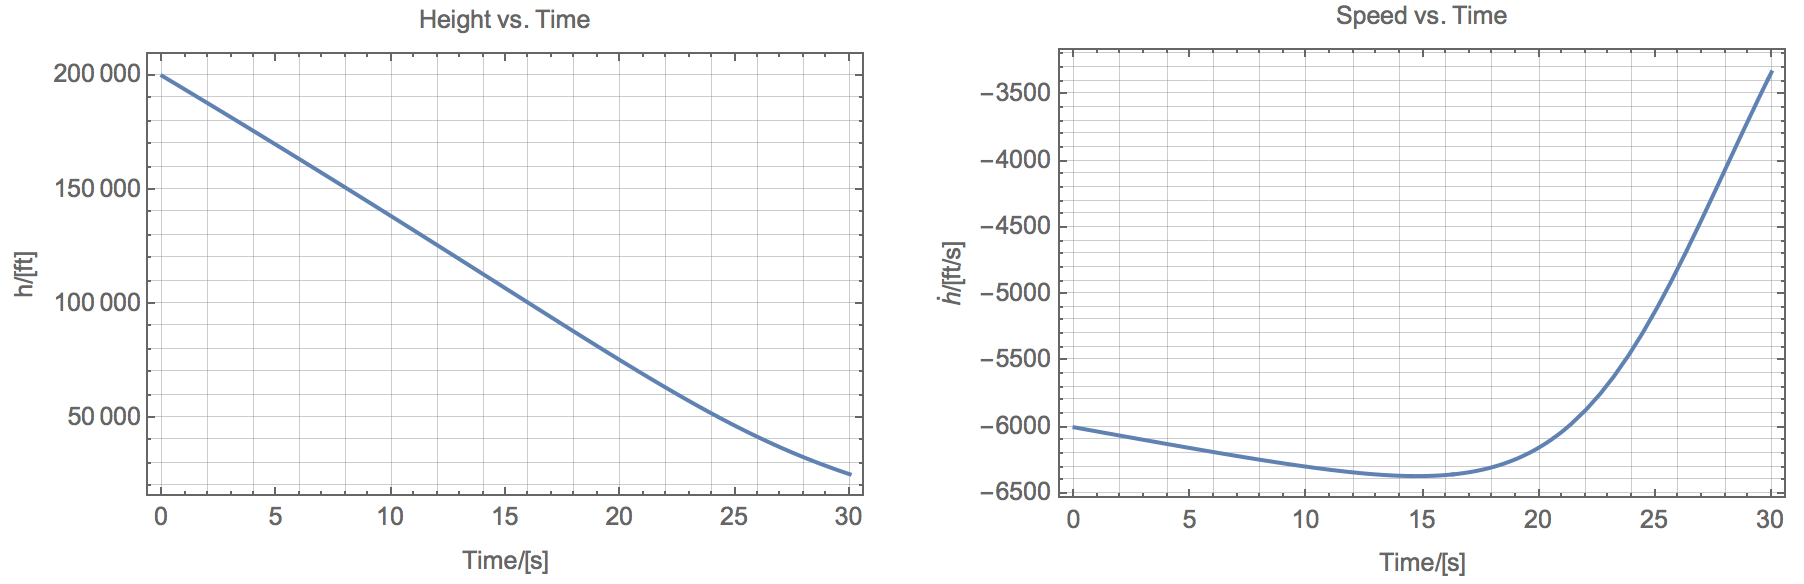
\includegraphics[width=.9\linewidth]{NDSolveFallingWithDrag.png}
\caption{\label{fig:orgparagraph1}
Trajectory of a falling object with drag}
\end{figure}

\noindent producing the results in figure \ref{fig:orgparagraph1}.
These results are indistinguishable from those in the reference.

\subsection{Stream Solver}
\label{sec:orgheadline6}

We can write the same differential equation as a lazy stream, which uses only
constant memory. Thus, it is suitable for the internals of a Kalman filter. We
implement the integrator as an accumulator function for a \texttt{foldStream} from
paper 3\footnote{B. Beckman, \emph{Kalman Folding 3: Derivations}, to appear.} which produces all intermediate results as a new stream:

\begin{verbatim}
foldStream[f_, s_, Null[]] := (* acting on an empty stream *)
  {s, Null}; (* produces a singleton stream containing 's' *)
foldStream[f_, s_, {z_, thunk_}] :=
  (* pass in a new thunk that recurses on the old thunk    *)
  {s, foldStream[f, f[s, z], thunk[]] &};
\end{verbatim}

The simplest integrator is the Euler integrator, which updates a state with its
derivative times a small interval of time: 

\begin{verbatim}
eulerAccumulator[{t_, x_}, {dt_, t_, Dx_}] :=
  {t + dt, x + dt Dx[x, t]};
\end{verbatim}

This is a binary function that takes two compound arguments. The first is an
instance of the accumulation type: a pair of a time \texttt{t} and a (usually compound)
state \texttt{x}. The second is an element of the input stream, a triple of a time
differential \texttt{dt}, the same time \texttt{t} that appears in the first argument, and a
function \texttt{Dx} that computes the derivative of the state given the state and the
time as \texttt{Dx[x,t]}. 

Folding this integrator over the streamed differential equation produces a
streamed solution. The input stream must produce elements of the form
\texttt{\{dt, t, Dx\}} and, like all streams, contain a thunk that produces the rest of the
stream.\footnote{Wolfram's ampersand postfix operator can covert its operand into a thunk.}

\begin{verbatim}
dragDStream[Delta : {dt_, t_, Dx_}] :=
  {Delta, dragDStream[{dt, t + dt, Dx}] &};
\end{verbatim}

This bit contains nothing specific to our example, but just threads around the
integration inputs and increments time. It could be much more rich,
manipulating \texttt{dt} and \texttt{Dx} for speed or numerics (\emph{adaptive integration}).

The kernel of our differential equation is the derivative function \texttt{Dx}, which,
for our example, is

\begin{verbatim}
With[{g = 32.2, A = 0.0034, k = 22000., beta = 500.},
  dragD[{x_, v_}, t_] := {v, g (A Exp[-x/k] v^2/(2. beta) - 1)}];
\end{verbatim}

\noindent Integrating the differential equation for thirty seconds looks like this:

\begin{verbatim}
(* constants and initial conditions *)
With[{x0 = 200000., v0 = -6000., t0 = 0., t1 = 30., dt = .1},
 takeUntil[
  foldStream[
   eulerAccumulator,
   {t0, {x0, v0}},
   dragDStream[{dt, t0, dragD}]
   ], First[#] > t1 &]] (* predicate on first elements of solution *)
\end{verbatim}

The type of the result, here, is a lazy stream produced by \texttt{takeUntil} from the
lazy stream produced by \texttt{foldStream}. Because these streams are lazy, nothing
happens until we demand values for, say, plotting. The results are
indistinguishable from those in figure \ref{fig:orgparagraph1}. 

The arguments of \texttt{takeUntil} are a stream and a predicate. The result is a new
stream that pulls values from the original stream, applying the predicate until
it produces \texttt{True}. At that point, the rest of the stream returned by
\texttt{takeUntil} is empty, represented by invocation of the null thunk, \texttt{Null[]},
The implementation of \texttt{takeUntil} is in three overloads:

Given an empty stream and any predicate, produce the empty stream:

\begin{verbatim}
takeUntil[Null[], _] := Null[];
\end{verbatim}

Given a stream containing a value \texttt{v} and a tail \texttt{thunk}, return the empty
stream if the predicate evaluates to \texttt{True}:

\begin{verbatim}
takeUntil[{v_, thunk_}, predicate_] /; predicate[v] := Null[];
\end{verbatim}

Otherwise, recurse by invoking the \texttt{thunk} in the stream:

\begin{verbatim}
takeUntil[{v_, thunk_}, predicate_] :=
  {v, takeUntil[thunk[], predicate] &};
\end{verbatim}

\subsection{What's the Point?}
\label{sec:orgheadline7}

The point of this style of integration is that we can change three aspects of
the integration independently of one another, leaving the others verbatim,
without even recompilation, because we have un-nested and \emph{decomplected}\footnote{``Decomplecting'' is a term coined by Rich Hickey for un-braiding and
un-nesting bits of software.} these aspects:
\begin{enumerate}
\item the integrator
\item sophisticated adaptive treatments of the time increment \texttt{dt} and derivative function \texttt{Dx}
\item the internals of the derivative function \texttt{Dx}
\end{enumerate}

For example, should Euler integration prove inadequate, we can easily substitute
second- or fourth-order Runge-Kutta integrators. The only requirement is that an
integrator must match the integrator's functional interface:

\begin{verbatim}
rk2Accumulator[{t_, x_}, {dt_, t_, Dx_}] :=
  With[{dx1 = dt Dx[x, t]},
   With[{dx2 = dt Dx[x + .5 dx1, t + .5 dt]},
    {t + dt, x + (dx1 + dx2)/2.}]];
rk4Accumulator[{t_, x_}, {dt_, t_, Dx_}] :=
  With[{dx1 = dt Dx[x, t]},
   With[{dx2 = dt Dx[x + .5 dx1, t + .5 dt]},
    With[{dx3 = dt Dx[x + .5 dx2, t + .5 dt]},
     With[{dx4 = dt Dx[x + dx3, t + dt]},
      {t + dt, x + (dx1 + 2. dx2 + 2. dx3 + dx4)/6.}]]]];
\end{verbatim}

Decomplecting these bits also makes them easier to review and verify by hand
because dependencies are lexically localized, making expressions smaller, easier
to memorize and to find on a page.

\subsection{Gain and Covariance Updates}
\label{sec:orgheadline8}

For gains and covariances, we need the best linear approximation of the
equations of motion so that we have an expression that structurally resembles equation
\ref{eqn:state-space-form}. When there are no disturbances,
\(\mathbold{G}\,\mathbold{u}=\mathbold{0}\) and the solution of the linear
equation \(\mathbold{\dot{x}}=\mathbold{F}\,\mathbold{x}\) also satisfies
\(\Delta\mathbold{\dot{x}}=\mathbold{F}\,\Delta\mathbold{x}\) for small
differences \(\Delta\mathbold{\dot{x}}\) and \(\Delta\mathbold{x}\). We seek a
similar form for our nonlinear equations of motion because we can linearize
them around small differences \(\Delta{h}\) and \(\Delta{\dot{h}}\):

\begin{equation}
\begin{bmatrix} \Delta \dot { h } \\ \Delta \ddot { h }
\end{bmatrix}
=
\begin{bmatrix}
\underset {  }{ \frac { \partial \dot { h }  }{ \partial h }  }  &
\underset {  }{ \frac { \partial \dot { h }  }{ \partial \dot { h }  }  }  \\
\frac { \partial \ddot { h }  }{ \partial h }  &
\frac { \partial \ddot { h }  }{ \partial \dot { h }  }
\end{bmatrix}
\begin{bmatrix}
\Delta h \\ \Delta \dot { h }
\end{bmatrix} 
=
\mathbold{F}(\mathbold{x}=[h\,\dot{h}]^\intercal) \cdot
\begin{bmatrix}
\Delta h \\ \Delta \dot { h }
\end{bmatrix} 
\end{equation}

\noindent 
Thus, with
\(k=22,000\,\left[\textrm{ft}\right]\), the e-folding height of the atmosphere,
and \(A=0.0034\,[\textrm{slug}/{{\textrm{ft}}^3}]\) for the density of
air\footnotemark[7]{} at \(h=0\),
our linearized system-dynamics matrix is

\begin{equation}
\mathbold{F}(\mathbold{x}) =
\begin{bmatrix}
\underset {  }{ 0 }  &
\underset {  }{ 1 }  \\
\frac{-A g {\dot{h}}^2 e^{{h}/{k}}}{2 \beta  k}  &
\frac{A g {\dot{h}} e^{{h}/{k}}}{\beta }
\end{bmatrix}
\end{equation}

We need \(\mathbold{\Phi}=e^{\mathbold{F}t}\) to propagate solutions forward,
because, if
\(\mathbold{\dot{x}}=\mathbold{F}\,\mathbold{x}\), then
\(e^{\mathbold{F}t}\,\mathbold{x}\)(t) effects a Taylor series. To first order, 

\begin{align}
\notag
\mathbold{x}(t+\delta{t}) &= e^{\mathbold{F}\,\delta{t}}\,\mathbold{x}(t) \\
\label{eqn:expand-f}      &\approx \left(\mathbold{1} + \mathbold{F}\,\delta{t}\right)\,\mathbold{x}(t) \\
\notag                    &= \mathbold{x}(t) + \mathbold{F}\,\mathbold{x}(t)\,\delta{t} \\
\notag                    &\approx \mathbold{x}(t) + \mathbold{\dot{x}}(t)\,\delta{t}
\end{align}

\noindent First-order expansions turn out to be enough, so
we take \(\mathbold{\Phi}(\delta{t})=\mathbold{1}+\mathbold{F}\,\delta{t}\) for
our propagator matrix. 

We compute the gains and covariances as in equations
\ref{eqn:covariance-propagation-equation}, 
\ref{eqn:kalman-gain-definition}, and
\ref{eqn:kalman-denominator-definition}:

\begin{align}
\mathbold{P}
&\leftarrow
\mathbold{\Xi}+
\mathbold{\Phi}\,
\mathbold{P}\,
\mathbold{\Phi}^\intercal
\end{align}

\noindent where \(\Xi\), integral of the process noise, is 

\begin{equation}
\left(\sigma_\xi\right)^2\cdot
\begin{bmatrix}
 \underset{}{\frac{{\delta t}^3}{3}}
&
 \underset{}{{{{\mathbold{F}_{22}}} {\delta t}^3}/{3}+\frac{{\delta t}^2}{2}}
\\
 {{{\mathbold{F}_{22}}} {\delta t}^3}/{3}+\frac{{\delta t}^2}{2} 
&
 {{{\mathbold{F}_{22}}}^2 {\delta t}^3}/{3}+{{\mathbold{F}_{22}}} {\delta t}^2+{\delta t}
\end{bmatrix}
\end{equation}

\noindent with matrix element \(\mathbold{F}_{22}\) evaluated at the current state
\(\mathbold{x}\).

\section{Concluding Remarks}
\label{sec:orgheadline10}

It's easy to add system dynamics to a static Kalman filter. Expressed as the
accumulator function for a fold, the filter is decoupled from the environment in
which it runs. We can run exactly the same code, even and especially the same
binary, over arrays in memory, lazy streams, asynchronous observables, any data
source that can support a \emph{fold} operator. Such flexibility of deployment allows
us to address the difficult issues of modeling, statistics, and numerics in
friendly environments where we have large memories and powerful debugging tools,
then to deploy with confidence in unfriendly, real-world environments where we
have small memories, asynchronous, real-time data delivery, and seldom more than
logging for forensics.
Emacs 24.5.1 (Org mode 8.3.4)
\end{document}